\section{Mechanistic illustrations: from a solvable model to real data}

\label{2605:sec:real-data}
For this section, codes are available at
\url{https://github.com/IdePHICS/Neural-LoFi-Theory}. 

\begin{figure}
    \centering
    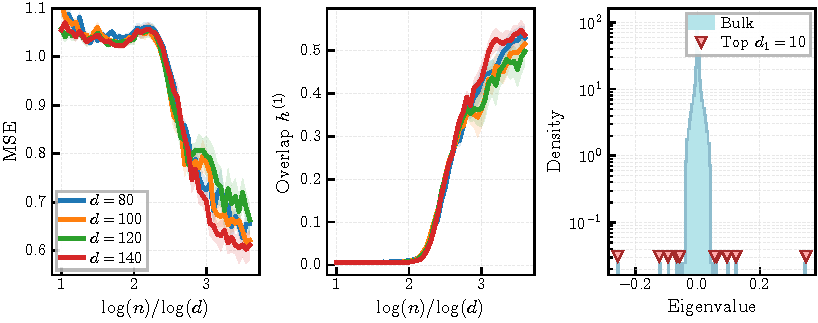
\includegraphics[width=\linewidth]{figs/rf_synthetic_model}
    \caption{
    \textbf{Neural LoFi in a mathematically solvable model}: 
    We used data generated by the two-level target Eq.\eqref{2605:model}, with ($k=2$), latent dimension $d_1=\lfloor d^\epsilon\rfloor$, $\epsilon=\tfrac12$, and final readout $g^\star(t)=\tanh(t)$, learned by a Neural LoFi approach. For $d\in\{80,100,120,140\}$, we use first-layer random-feature widths $p_1\in\{20000,30000,40000,50000\}$ and second-layer widths $p_2\in\{512,768,1024,1280\}$. The final one-dimensional non-linearity is fitted with a polynomial kernel of maximal degree $5$, using ridge regularization $10^{-6}$ and kernel regularization $10^{-4}$. \textbf{Left:} Mean Squared Error (MSE) of the final predictor as a function of $\alpha$, for input dimensions $d\in\{80,100,120,140\}$. Notice the drop at the predicted sample complexity for feature learning $n \propto d^{2.5}$.
    \textbf{Center:} Overlap between the recovered first-layer representation $\widehat h^{(1)}$ and the ground-truth latent variables $h^{(1)}$.   
    \textbf{Right:} Spectrum of the first random-feature spectral operator $\widehat C_1$ for $d=100$ at $\alpha=3$, where $d_1=10$, showing the emergent informative features.
    }
    \label{2605:fig:rf_theoretical}
\end{figure}

\subsection{A solvable model}
\label{2605:sec:the model}
We first consider a toy model in which the full Neural LoFi mechanism can be inspected mathematically, that illustrates the salient feature discussed in the former section: {\it emergence} and {\it low-degree compositionality}. Following the hierarchical polynomial constructions of
\cite{nichani2023provable,wang2024learning,fu2025learning,tabanelli2026deep}, let $\bm x\sim \mathcal N(0,I_d)$ and generate labels through a planted compositional hierarchy
$
\bm x
\;\longrightarrow\;
\bm h^{(1)}(\bm x)
\;\longrightarrow\;
h^{(2)}(\bm x)
\;\longrightarrow\;
y$. Let $H_k(\bm x)$ denote the degree-$k$ Hermite feature vector of the input. We plant $d_1=d^\varepsilon$ random directions
$\bm A_1^{(1)},\ldots,\bm A_{d_1}^{(1)}$ in this degree-$k$ feature space, together with a random symmetric matrix
$\bm A^{(2)}\in\mathbb R^{d_1\times d_1}$ acting on the first hidden layer. The hidden variables are
\begin{equation}
    h_i^{(1)}(\bm x)
    =
    \big\langle \bm A_i^{(1)}, H_k(\bm x)\big\rangle,
    \qquad i=1,\ldots,d_1,
\end{equation}
and the second representation is a quadratic function of these variables,
\begin{equation}
    h^{(2)}(\bm x)
    =
    \big\langle \bm A^{(2)}, H_2(\bm h^{(1)}(\bm x))\big\rangle,
    \qquad
    y = g^\star(h^{(2)}(\bm x)).\label{2605:model}
\end{equation}
While the target is high-degree as a function of the input, it factors into low-degree transitions: $\bm h^{(1)}$ is degree-$k$ in $\bm x$, and $h^{(2)}$ is quadratic in $\bm h^{(1)}$. This is why the model is useful for illustrating both the advantage of feature learning and the advantage of depth: A fixed kernel or random-feature method \cite{mei2022generalizationerror} sees only the composed map $\bm x\mapsto y$; if $g^\star$ contains a degree-$r$ component, then for $k=2$ this includes degree-$4r$ structure in the input. No learning whatsoever would arise before at least $n=O(d^4)$ data just to beat a random guess!

A two-layer feature learner can already improve on such a one-shot approach by recovering the first hidden representation $\bm h^{(1)}$, but the remaining target is still a nonlinear function of the $d_1=d^\varepsilon$ latent variables, and thus we still face the curse of dimension (over $d_1$ instead of $d^\varepsilon$).

This is where the multi-layer approach solve the problem: A second feature-learning step provides the depth advantage: once $\bm h^{(1)}$ is recovered, the next hidden variable $h^{(2)}$ is only a quadratic spectral problem in dimension $d_1$, followed by a one-dimensional readout. The model realizes the separation identified in \cite{tabanelli2026deep}, but now with Neural LoFi itself: Each layer lowers the effective degree of the remaining task by making the next hidden variable visible through a low-degree statistic. The final target is therefore learned by Neural LoFi progressively, and efficiently, building the correct intermediate representation, rather than by fitting the full high-degree map $\bm x\mapsto y$ in one shot. 

Appendix~\ref{2605:app:th_rf} provides the corresponding mathematical theorems and synthetic experiments, demonstrating feature emergence at the predicted sample scales (Eq.\ref{2605:eq:lofi-emergence-threshold}), spectral outlier formation, alignment with the planted features, and recovery of the final compositional target. 

We thus refer to Appendix~\ref{2605:app:th_rf} for more details  and just briefly illustrate here the performance of Neural LoFi in Fig.~\ref{2605:fig:rf_theoretical}: The function becomes learnable at \(n\gg D_k d_1=O(d^{k+\varepsilon})\), which, in the quadratic case used in the experiments, is \(n\gg d^{2+\varepsilon}\). Around this scale, the Neural LoFi estimator simultaneously shows a drop in prediction error, a sharp increase in overlap with the planted representation, and the separation of the leading eigenvalues from the spectral bulk (see right panel in Fig.~\ref{2605:fig:rf_theoretical} as well as Fig.~\ref{2605:fig:rf_spectrum} showing the emergence of learned features in the first layer in Appendix). 

%Here, the label-weighted Neural LoFi operator has a transparent signal-plus-noise structure making its analysis accessible mathematically: At the first layer, its population part is aligned with the span of the planted directions $\{\bm A_i^{(1)}\}_{i=1}^{d_1}$, while finite samples create a spectral noise bulk. As $n$ increases, the informative directions separate from this bulk through BBP/EA-type transitions; and the associated eigenvectors recover the hidden features.
%Once this first representation is recovered, the second stage $h^{(2)}$ becomes visible through another low-degree spectral problem. 


\begin{figure}
    \centering
    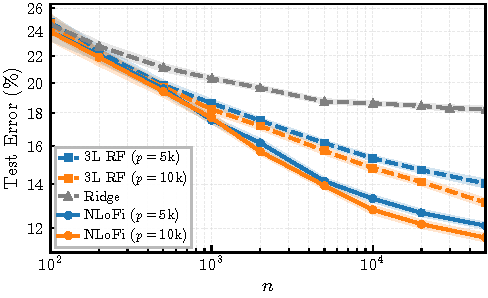
\includegraphics[width=0.6\linewidth]{figs/error_vs_ntrain_cifar10_layers_3_relu_p5000_10000}
    
    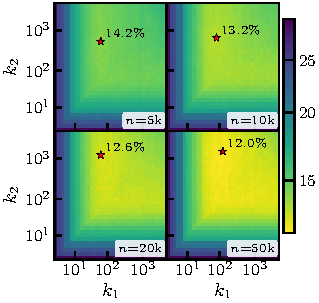
\includegraphics[width=0.37082\linewidth,height=0.37082\linewidth]{figs/k1k2_heatmap_ntrain_grid_cifar10_layers3_p5000_relu_ntrain5000_10000_20000_50000_error}
    \caption{
    \emph{Fully connected Neural LoFi on the CIFAR-10 animal-vs.-vehicle task.}
    \textit{Left:} Test error vs number of training samples for ridge regression, three-layer random features, and Neural LoFi, with projection dimensions $p=1\mathrm{k}$ and $p=5\mathrm{k}$.
    \textit{Right:} Test error over the number of retained features $(k_1,k_2)$ in the first two LoFi layers, for different training-set sizes and fixed projection dimension $p=5\mathrm{k}$. Stars indicate the best point in each grid.
    }
    \label{2605:fig:heatmaps}
\end{figure}


\subsection{Fully connected networks (FCN)} 
We now focus on experiments on real data, intended as mechanistic illustrations of the theory, not as a claim that Neural LoFi is a competitive training algorithm. Fig.\ref{2605:fig:heatmaps} (FCN on CIFAR-10 \cite{krizhevsky2009learning}) illustrates two qualitative predictions: i) the label-weighted LoFi operator extracts useful directions beyond those available to fixed random features, leading to a consistent improvement over ridge and random-feature baselines. ii) feature selection is non-trivial: the best test error is not always achieved by keeping the largest number of features. As the sample size grows, the optimal number of retained features increases or remains stable, matching the signal-to-noise picture in which weaker directions become accessible with more data.\begin{figure}\begin{center}
    
    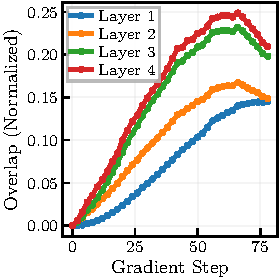
\includegraphics[width=0.35\textwidth]{figs/alignment_plot_fro}
  \end{center}
  \caption{
  Layer-wise normalized overlap 
  (see App.~\ref{2605:app:gd-feature-alignment}) between features learned by SGD at different steps with the Neural LoFi representation, for a four-layer FCN on CIFAR-10.
  }
   
  \label{2605:fig:gradient-alignment}
\end{figure}



We also compare Neural LoFi with a standard back-propagation approach: The overlap in Fig.~\ref{2605:fig:gradient-alignment} appears to grow during the early stages of training, indicating that LoFi approximates the initial feature-discovery phase of SGD. This is further supported by the aforementioned Fig.~\ref{2605:fig:gd-lofi-comparison}, that shows  direct test-error comparisons between GD and Neural LoFi. At later times, the alignment plateaus or decreases, suggesting that backpropagation eventually moves beyond the one-step LoFi approximation and learns features involving richer training dynamics. 

Most directly, Fig.~\ref{2605:fig:sample-complexity-pred} tests the feature-emergence criterion of Eqs.~\eqref{2605:eq:lofi-emergence-threshold} and~\eqref{2605:eq:emergence_feature}. We compare each eigenvector learned from \(n\) samples with a large-sample reference eigenvector, and mark the predicted emergence thresholds. The overlap curves rise close to these thresholds, showing that the effective-dimension criterion predicts the sample scale at which individual task-relevant directions ("concepts") become learnable. Additional details on this experiment are given in App.~\ref{2605:app:feature-recovery}; further numerical evidence, including spectra of the $\widehat C$ operator and experiments with the infinite-width Neural LoFi kernel, is reported in App.~\ref{2605:app:numerical-extra}.



\begin{figure}
    \centering
    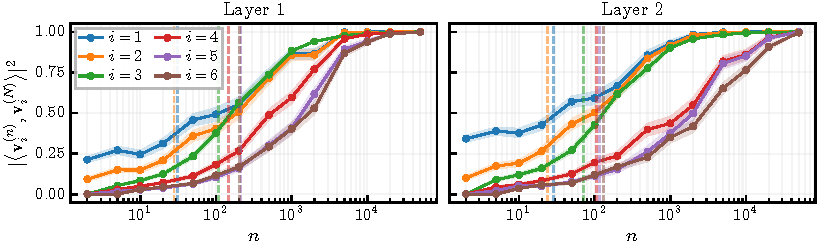
\includegraphics[width=\linewidth]{figs/main_overlap_per_eigvec_summary_whit_1x2_paper_v4_k1_6_n2}
    \caption{
    \textbf{Predicting when individual features emerge on CIFAR-10.}
    For a three-layer fully connected Neural LoFi model on the CIFAR-10 animal-vs.-vehicle task, we track the squared overlap
    $|\langle v_i^{(n)},v_i^{(N)}\rangle|^2$
    between eigenvectors estimated from \(n\) samples and large-sample reference eigenvectors computed with \(N=60{,}000\) samples. Curves show mean \(\pm\) SEM over 100 random subsamples at fixed random features. Dashed vertical lines indicate the predicted emergence thresholds \(n_\ell^i\) from \eqref{2605:eq:lofi-emergence-threshold},\eqref{2605:eq:emergence_feature}
    (for further details, see Eq.~\eqref{2605:eq:real-data-emergence-estimate} in Appendix). The sharp rise of each overlap near its predicted threshold shows that the effective-dimension criterion predicts when individual task-relevant directions become learnable.
    }
    \label{2605:fig:sample-complexity-pred}
\end{figure}


\subsection{Convolutional networks (CNN)}
Neural LoFi is not restricted to fully connected architectures: the moment operator can be built in the feature space exposed by the architecture. This makes it natural to incorporate structural inductive biases such as locality, weight sharing, equivariance, or graph structure, in the spirit of geometric deep learning~\cite{bronstein2021geometric}. Here, we consider convolutional networks.
Let $\bm z_{\ell-1}(\bm x_\mu)\in\mathbb R^{s_\ell\times p_{\ell-1}}$ denote the input features to layer $\ell$, where $s_\ell$ is the number of spatial locations and $p_{\ell-1}$ is the number of channels. We define the operator in channel space as:
\begin{equation}
    \widehat{\bm C}^{(\ell)}
    \coloneqq
    \frac{1}{n s_\ell}
    \sum_{\mu=1}^n
    \sum_{j=1}^{s_\ell}
    y_\mu\,
    \bm z_{\ell-1}(\bm x_\mu)_j
    \bm z_{\ell-1}(\bm x_\mu)_j^\top .
\end{equation}
The top eigenvectors of $\widehat{\bm C}^{(\ell)}$ define the task-relevant channel directions retained at layer $\ell$; the resulting features are then passed through the same fixed random lifting used by Neural LoFi. 


We remind that Fig.~\ref{2605:fig:gd-lofi-comparison} showed how similar direct GD optimization is to Neural LoFi at early training time. The convolutional experiment also gives the most direct visual evidence for low-degree compositionality. Applying the LoFi operator directly to pixels already recovers familiar low-level visual features: a leading color-sensitive direction, followed by localized contrast and edge-like filters. Several later filters resemble finite-difference or Laplacian-like stencils, echoing classical edge-filter emergence in natural image models~\cite{olshausen1996emergence} and the early filters learned by CNNs trained with gradient descent~\cite{krizhevsky2012imagenet,zeiler2014visualizing,radhakrishnan2024mechanism}. 
In appendix, we further show in
Fig.~\ref{2605:fig:sample-complexity-pred-conv}  the feature-emergence criterion of Eqs.~\eqref{2605:eq:lofi-emergence-threshold} and~\eqref{2605:eq:emergence_feature} for GNN, as we did for FCN in Fig.\ref{2605:fig:sample-complexity-pred}.

\begin{figure}
    \centering
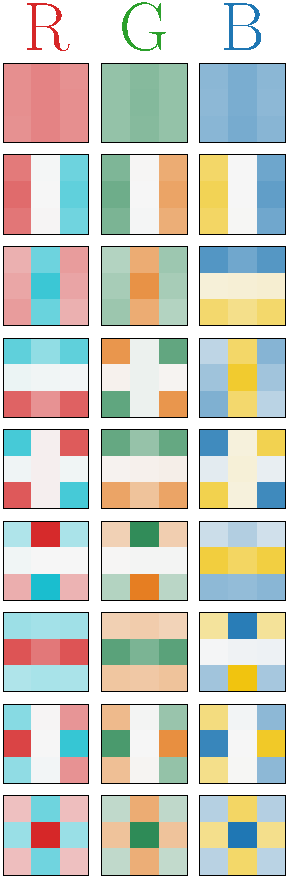
\includegraphics[width=2cm,height=6.25cm]{figs/cifar10_filters}
    
    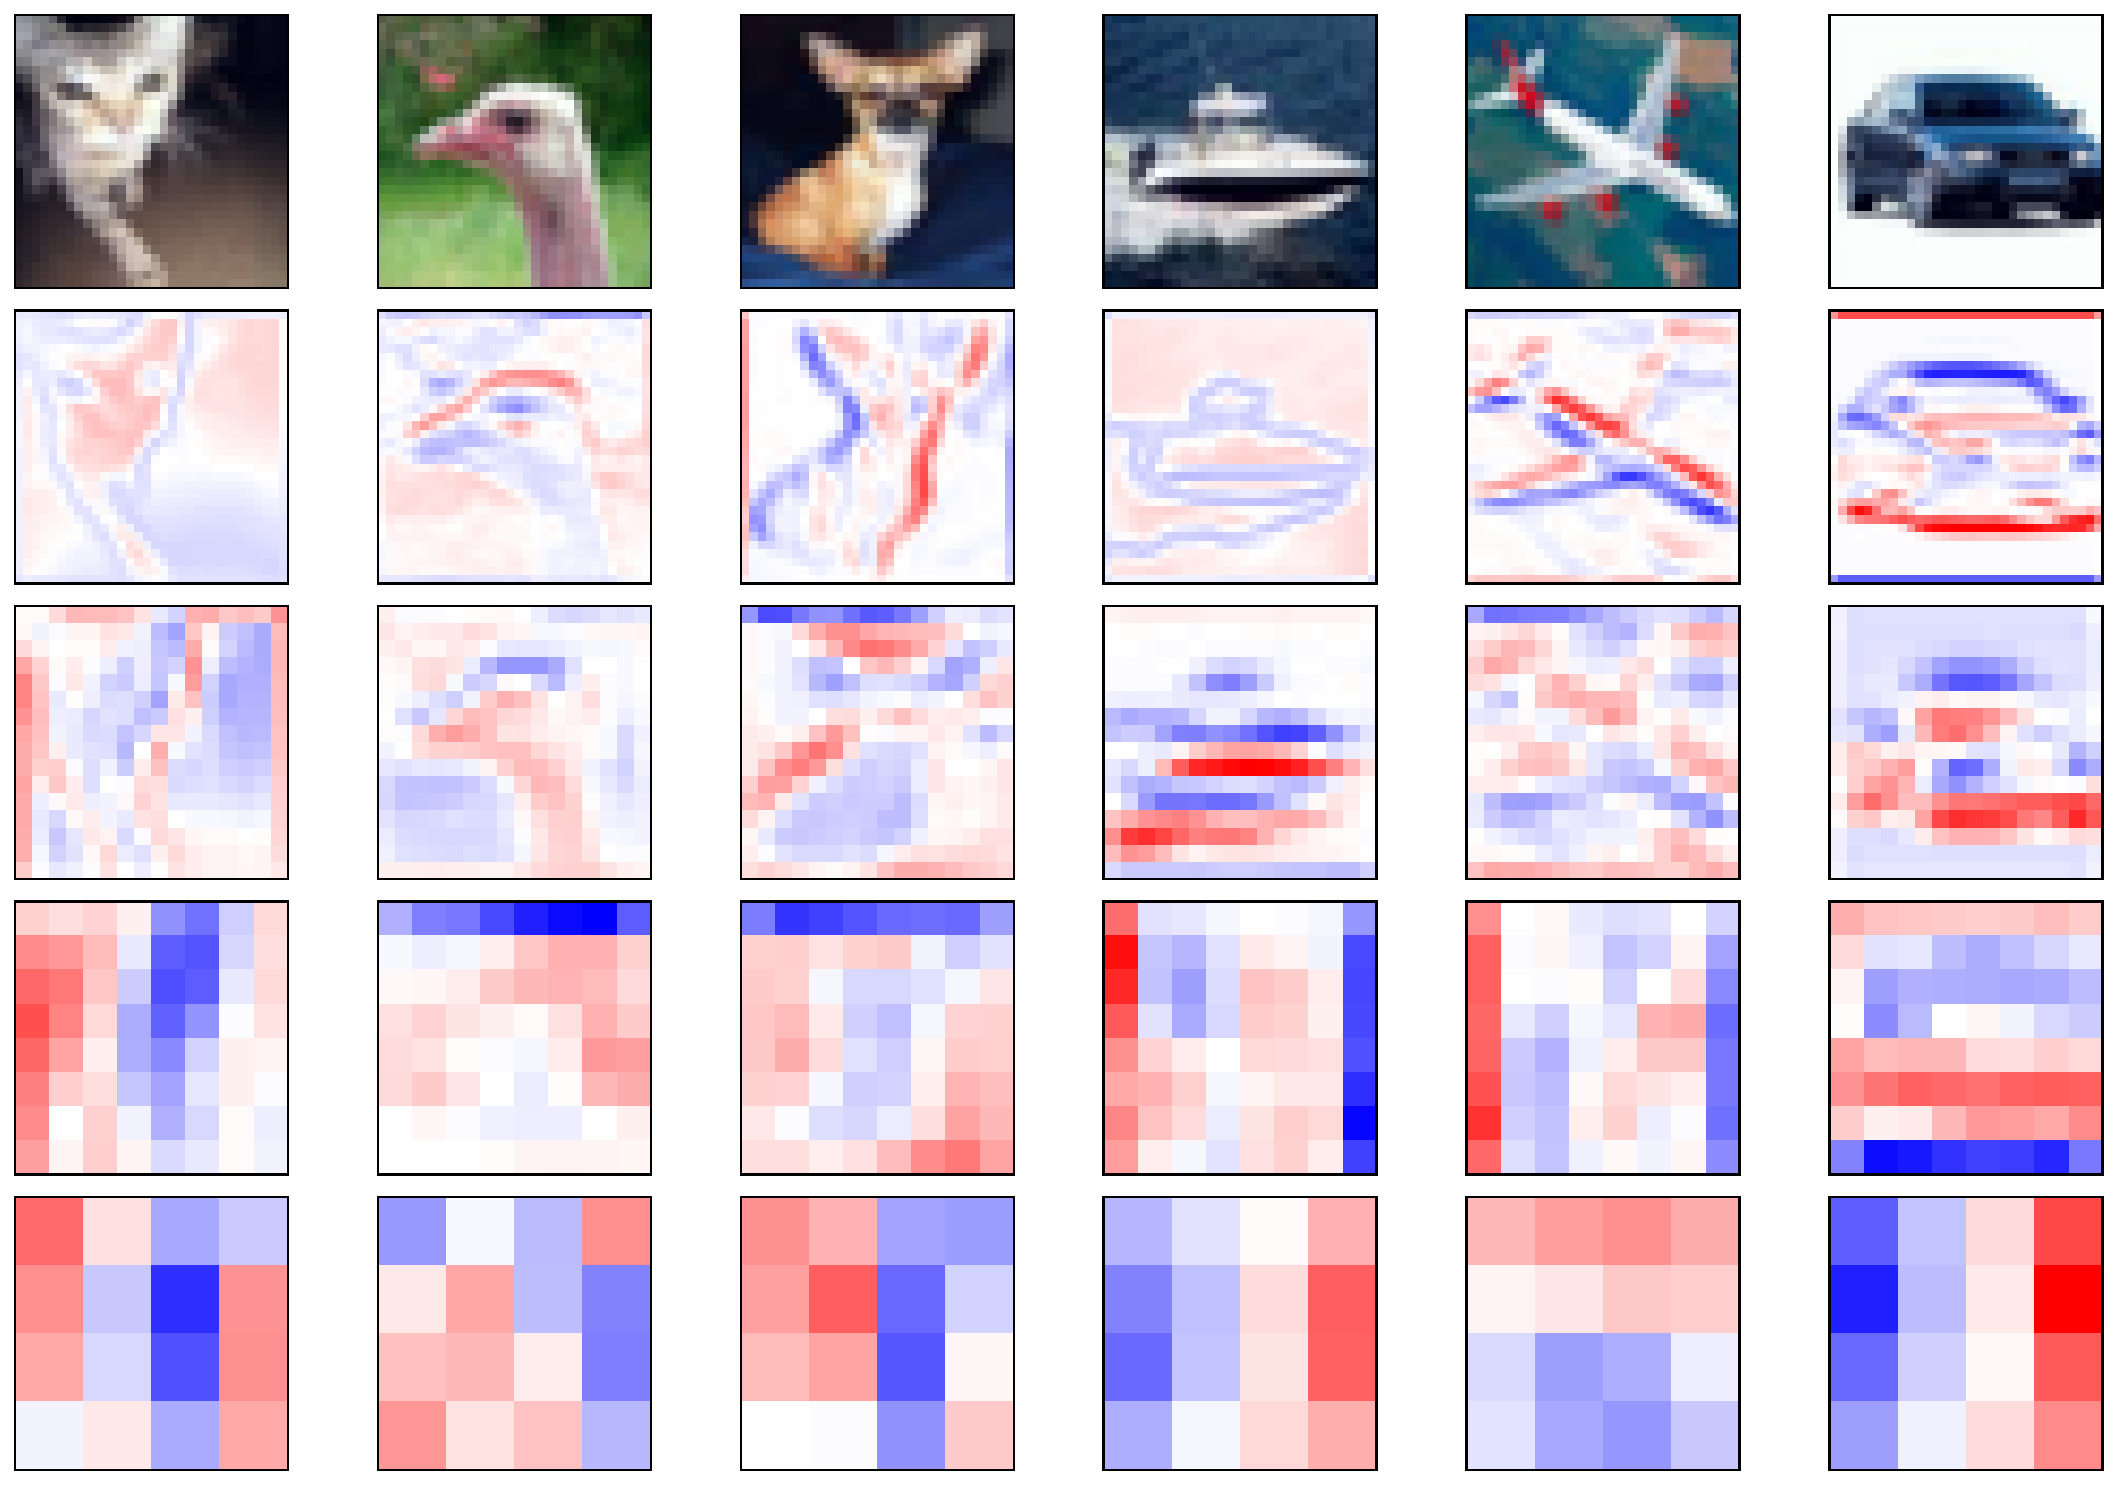
\includegraphics[width=6.9cm,height=6.25cm]{figs/rank_06_definitive_activations}
  \caption{
  Neural LoFi with convolutional layers on the CIFAR-10 animal-vs.-vehicle task. Neural LoFi recovers the usual structures and edge detectors associated to GNN {\it without backpropagation or end-to-end optimization}
  \textit{Left:} Top first-layer filters obtained from the three RGB input channels.
  \textit{Right:} Activations of the sixth LoFi feature on test images at successive depths; top row shows the input images, lower rows  the corresponding activation maps.
  }
  \label{2605:fig:cnn-filter-activations}
\end{figure}


Strikingly, these salient visual structures emerge {\it without backpropagation or end-to-end optimization}: they are obtained simply by diagonalizing the Neural LoFi label-weighted moment operator. This shows that part of early visual feature learning is already captured by the low-degree supervised correlations emphasized by our theory. Depth then turns these simple local filters into more selective features. In Figure~\ref{2605:fig:cnn-filter-activations}, the same LoFi feature behaves like a generic edge or contrast detector at shallow depth, but becomes increasingly selective after successive LoFi layers, responding only to more structured spatial patterns. This is, again, the qualitative mechanism suggested by the theory: each layer extracts a low-degree task-correlated component from the current representation, and repeated extraction builds progressively more structured features. 
Additional  experiments (including the spectrum of the operators, and different datasets) are presented in App.~\ref{2605:app:numerical-extra}.
